\documentclass[a4paper]{article}
\usepackage[margin=2cm]{geometry}
\usepackage{graphicx}
\graphicspath{{Imagenes/}}
\usepackage{subfig}
\usepackage{float}

%\font\titleFont = cmr12 at 40pt
%\title{{\titleFont Trabajo Pr\'actico de Probabilidad y Estad\'istica}}
%\title{{\fontsize{30cm}{1cm}\selectfont Trabajo Pr\'actico de Probabilidad y Estad\'istica}}
\title{{\Huge Trabajo Pr\'actico de Probabilidad y Estad\'istica:
	\linebreak 
	Ley de los Grandes N\'umeros y el Teorema Central del L\'imite}}
\author{Buceta Diego, Springhart Gonzalo, Tasat Dylan}

\begin{document}
	\maketitle %Ponemos el título
	\thispagestyle{empty} %Sacamos el número de pie de página
	
	\newpage %Saltamos a la próxima página
	\setcounter{page}{1} %Reseteamos el contador
	
	%Ahora empieza el documento de verdad
	
	\section{Pre\'ambulo}
	La Ley de los Grandes N\'umeros y el Teorema Central del L\'imite son temas fundamentales de la probabilidad y la estad\'istica, sin embargo entender ambos no es trivial. Mediante este trabajo buscamos entender los conceptos de la Ley de los Grandes N\'umeros y el Teorema Central del L\'imite mediante ejercicios que ponen en evidencia el cumplimiento de ambos.
	
	\newpage
	
	\section{Primer Ejercicio}
	
	En este ejercicio, trabajamos con una variables aleatorias exponenciales todas con par\'ametro $\lambda = 2$. Con estas variables generamos 3000 experimentos de $n$ observaciones cada uno, es decir el primer experimento tiene una observaci\'on, el segundo dos y as\'i sucesivamente. 
	
Si tomamos la media de cada uno de los experimentos y la graficamos podermos ver que queda el siguiente gr\'afico:

	
	\begin{figure}[H]
		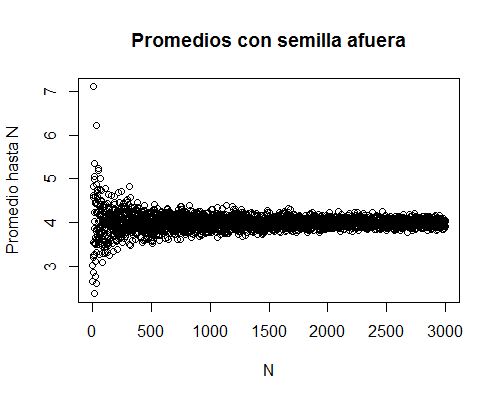
\includegraphics[scale=0.75]{grafico1}
		\centering
	\end{figure}

%	{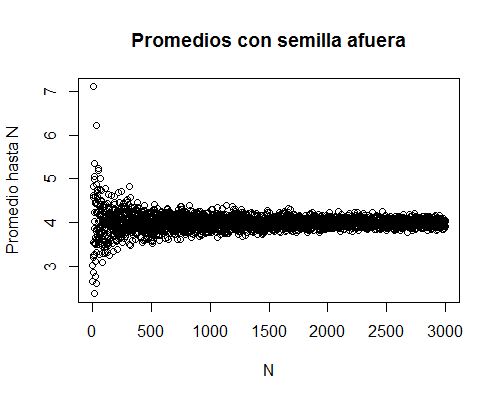
\includegraphics[scale=0.75]{grafico1}
%	\centering}
	
%	Se puede observar que el gr\'afico tiene una pinta similar al de una normal, esto nos sirve para ver una representaci\'on del Teorema Central del L\'imite, que dice que si se tienen $X_1,...,X_n$ variables aleatorias i.i.d. con esperanza $\mu$ y varianza $\sigma^2$ entonces si $n$ es lo suficientemente grande, la variable aleatoria $\bar{X} = \frac{1}{n}\sum_{i=1}^{n} X_i$ tiene aproximadamente una distribuci\'on $\mathcal{N}(\mu, \frac{\sigma^2}{n})$.

	Podemos observar en el gr\'afico como ocurre la Ley de los Grandes N\'umeros, a medida que crece la cantidad de observaciones, el resultado del experimento se acerca a la esperanza de una variable exponencial con par\'ametro $\lambda = 2$.  
	
%	\bigskip
%
%	\textbf{\large Diferencias de Gr\'aficos}
	
	\smallskip
	
	\subsection{Diferencias de Gr\'aficos}
	
	Como el t\'itulo ind\'ica, el gr\'afico anterior fu\'e computado en R seteando primero una semilla afuera de un ciclo for. Si a esa semilla la colocamos dentro del ciclo el gr\'afico mostrado cambia al siguiente
	
	
	\begin{figure}[H]
		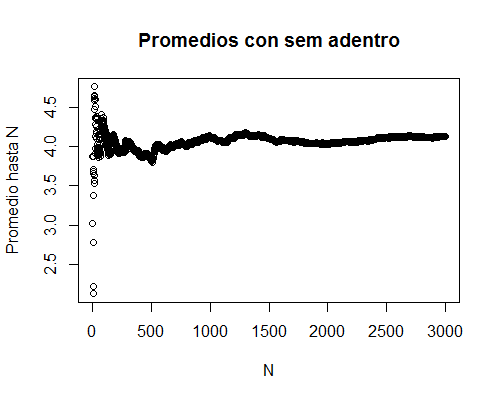
\includegraphics[scale=0.75]{grafico2}
		\centering
	\end{figure}
	
	Como se puede ver, los dos gr\'aficos son diferentes, \textquestiondown A qu\'e se debe \'esta diferencia? Se debe al modo en que R trabaja con las semillas al momento de generar datos al azar.
	
	En R al pedir que se genere un valor al azar, la \'unica forma de que ese valor siempre sea el mismo es setear la semilla antes de generarlo. Si se pide que se generen m\'as observaciones de las que se generaron antes, la \'unica observaci\'on distinta va a ser la final, es decir, si primero genero una variable con $n$ observaciones y despu\'es genero una nueva variable con $n+1$ observaciones, las primeras $n$ observaciones de esa nueva variable van a ser iguales a las $n$ de la anterior si seteo la misma semilla antes de generarla.
	En el segundo gr\'afico se grafican las medias calculadas de la misma forma que en el primer gr\'afico, pero en este caso, como la semilla esta dentro del ciclo for, las observaciones de cada experimento son las mismas, la \'unica diferencia es la cantidad de observaciones que tiene cada experimento.
	En este segundo gr\'afico tambi\'en se puede ver como las medias se empiezan a aproximar a la esperanza de la variable aleatoria exponencial cuando $n$ es grande.
	\newpage
	
	\section{Segundo Ejercicio}
	
	En \'este ejercicio vamos a poder apreciar la Ley de los Grandes N\'umeros, empezaremos guardando la media de dos observaciones de variables exponenciales 1000 veces, resultando en los siguientes gr\'aficos:
	
	\begin{figure}[H]
		\centering
		\subfloat{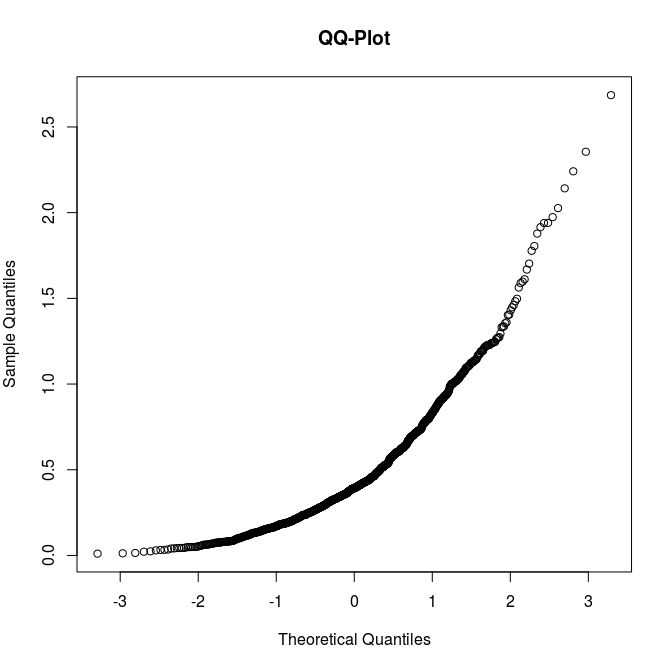
\includegraphics[scale = 0.3]{grafico3}}
		\hfill
		\subfloat{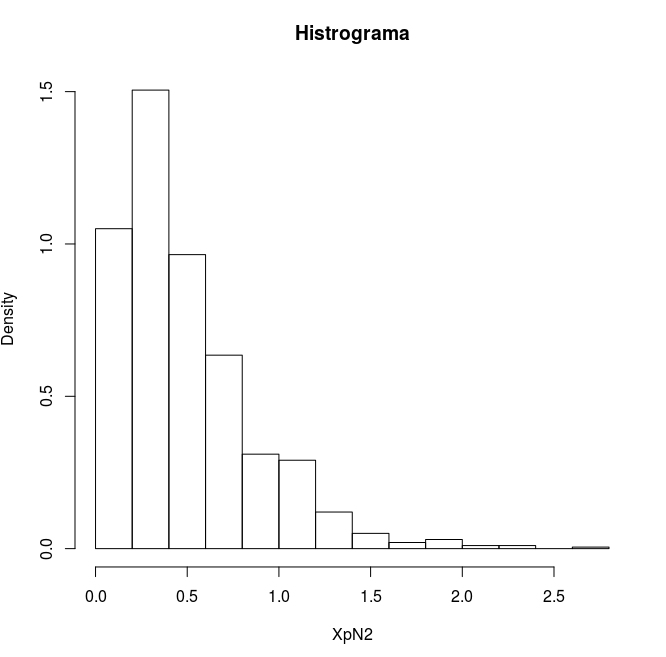
\includegraphics[scale = 0.3]{grafico4}}
		\hfill
		\subfloat{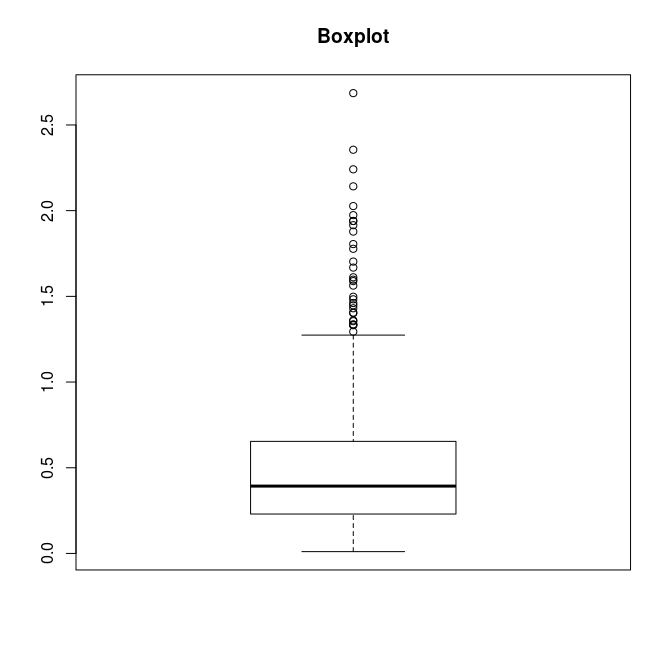
\includegraphics[scale = 0.3]{grafico5}}
	\end{figure}
	
	De los gr\'aficos podemos inferir que las medias no poseen una distribuci\'on normal, ya que el QQ-plot no se asemeja a una recta, en el histograma se ve que hay mayor concentraci\'n cerca de la media (aunque no necesariamente en la media), y tambi\'en podemos ver que hay una cantidad muy grande de "outliers" en el boxplot.
	
	Si aumentamos la cantidad de observaciones por muestra a 5 se obtienen estos gr\'aficos:
	
	\begin{figure}[H]
		\centering
		\subfloat{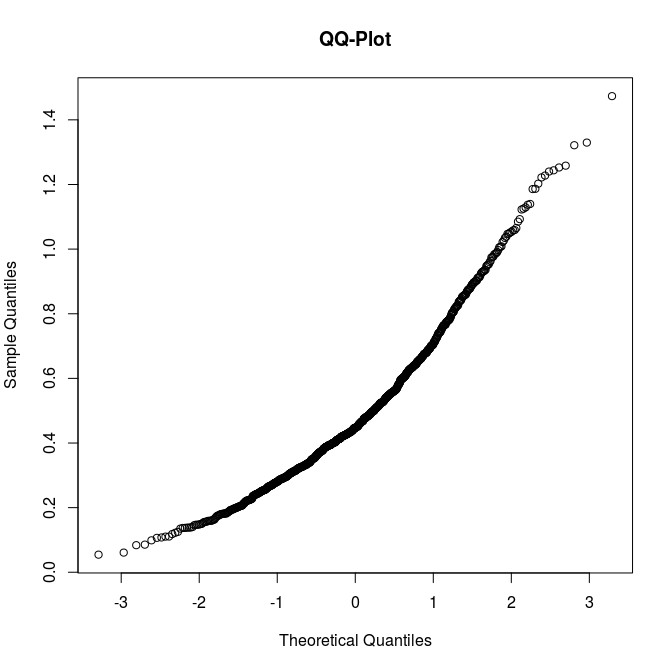
\includegraphics[scale = 0.26]{grafico6}}
	\end{figure}
	
	\begin{figure}[H]
		\centering
		\subfloat{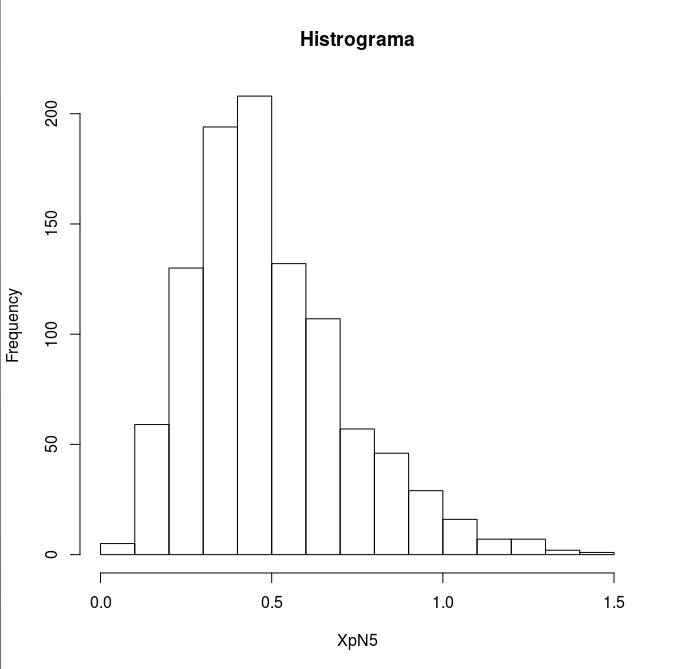
\includegraphics[scale = 0.3]{grafico7}}
		\hfill
		\subfloat{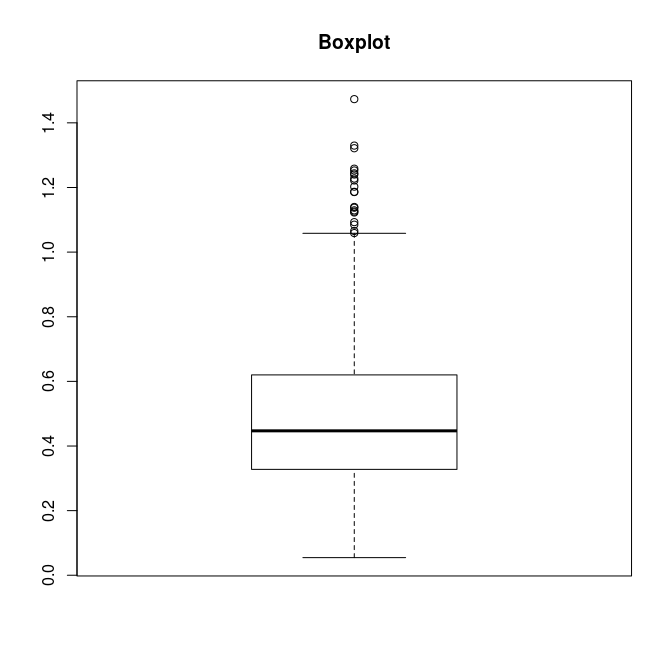
\includegraphics[scale = 0.3]{grafico8}}
	\end{figure}
	
	Se empiezan a notar los cambios de los gr\'aficos, en el QQ-plot vemos que los puntos se empiezan a parecer a una recta, en el histograma se ve que la concentraci\'on se acerca m\'as a la media, adem\'as tambi\'en se ve que en el boxplot se redujeron la cantidad de "outliers" que caen fuera del gr\'afico.
	
	Ahora si aumentamos la cantidad de observaciones a 30, los cambios se asent\'uan a\'un m\'as, resultando en los siguientes gr\'aficos:
	
	\begin{figure}[H]
		\centering
		\subfloat{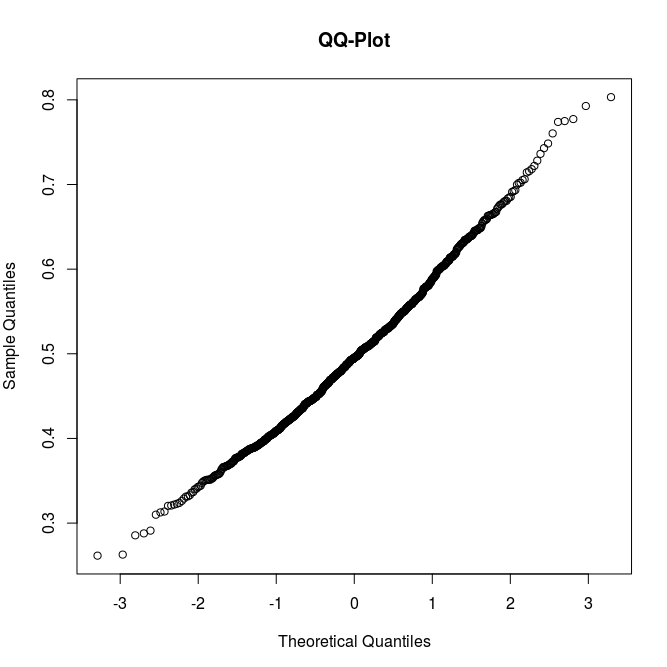
\includegraphics[scale = 0.3]{grafico9}}
		\hfill
		\subfloat{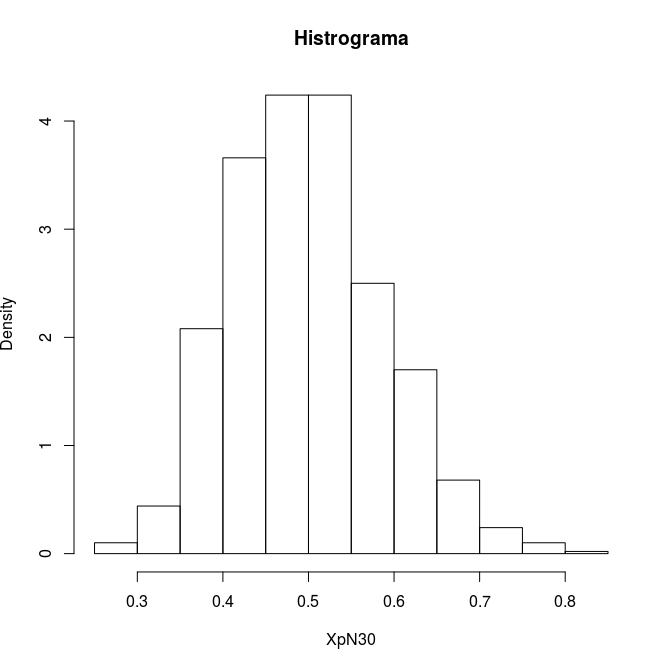
\includegraphics[scale = 0.3]{grafico10}}
		\hfill
		\subfloat{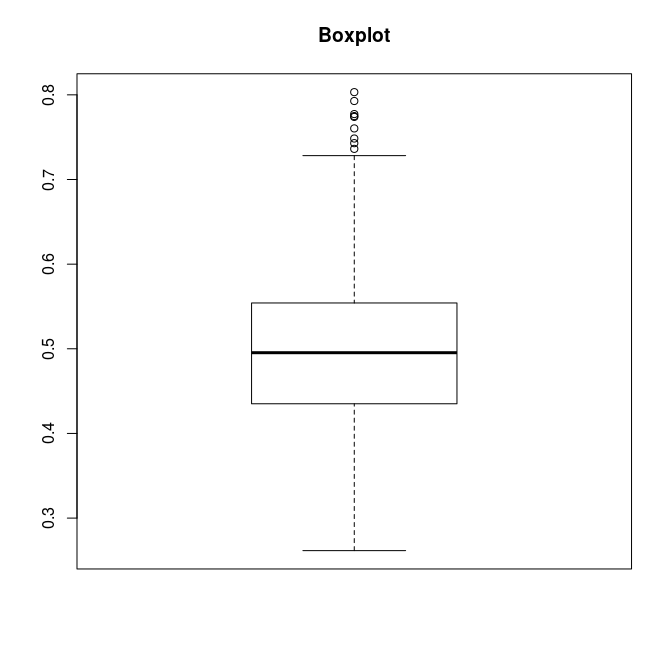
\includegraphics[scale = 0.3]{grafico11}}
	\end{figure}
	
	Se puede notar claramente en el QQ-plot que el gr\'afico se parece a una recta, indicando que la distribuci\'on de las medias puede ser normal, a su vez ahora el histograma tiene forma similar a un gr\'afico de una distribuci\'on normal y que el boxplot no s\'olo tubo otra disminuci\'on en la cantidad de "outliers" sino que tambi\'en esta m\'as centrado, de lo que podemos deducir mayor simetr\'ia en la distribuci\'on de las medias.
	
	Finalmente si aumentamos las observaciones a 500 por muestra, se obtienen estos gr\'aficos:
	
	\begin{figure}[H]
		\centering
		\subfloat{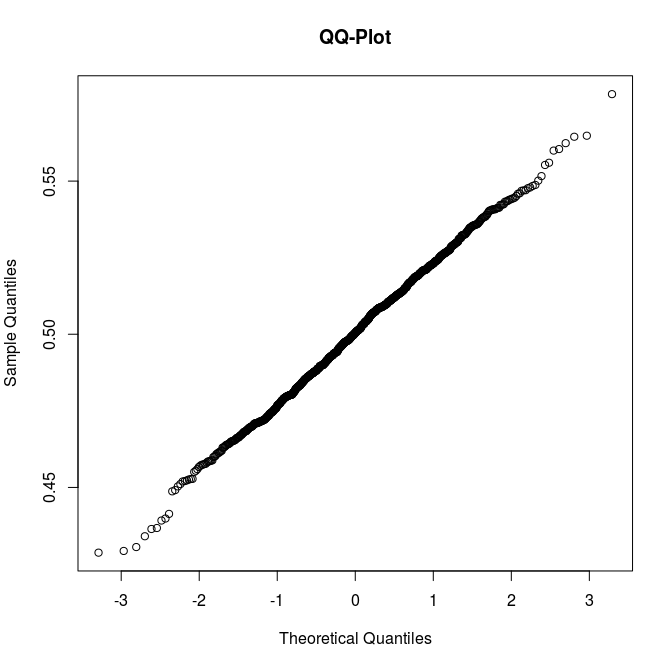
\includegraphics[scale = 0.3]{grafico12}}
		\hfill
		\subfloat{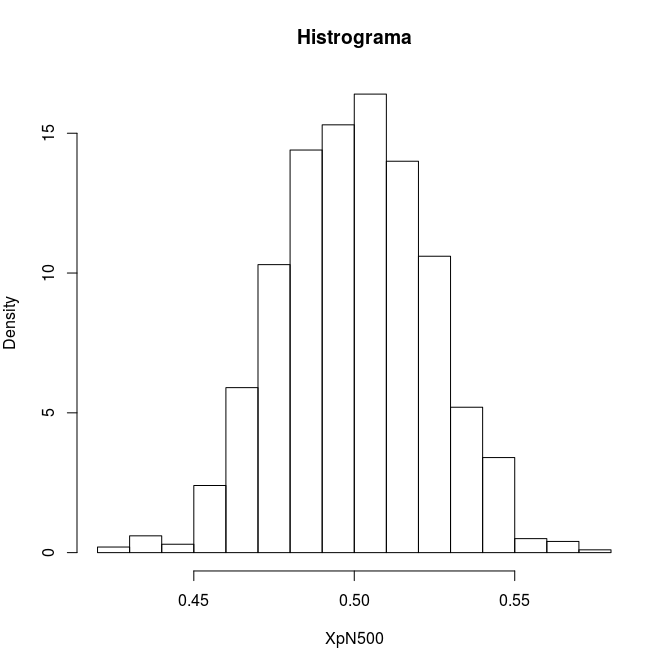
\includegraphics[scale = 0.3]{grafico13}}
		\hfill
		\subfloat{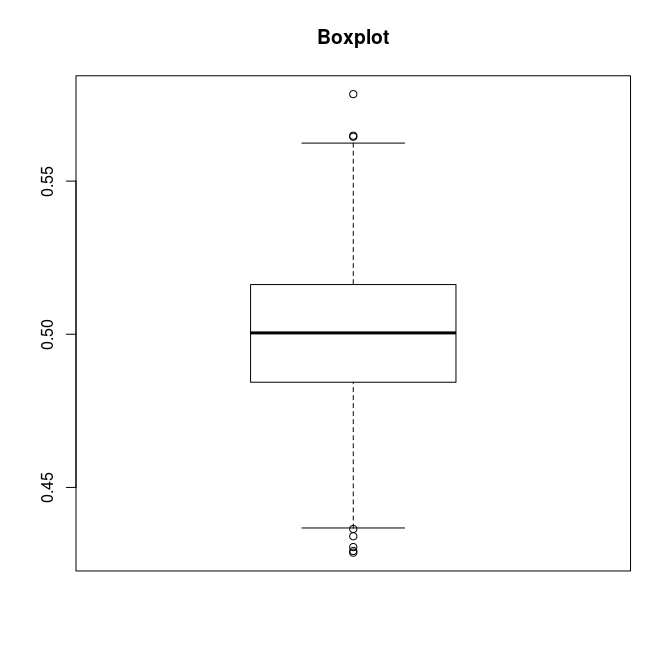
\includegraphics[scale = 0.3]{grafico14}}
	\end{figure}
	
	En estos gr\'aficos además de ver a\'un m\'as acentuaci\'on de las caracter\'isticas mencionadas anteriormente, podemos ver que la mayor\'ia de las medias cae cerca de la esperanza de las variables.
	Para marcar ese progreso podemos ver en conjunto los boxplot de los experimentos
	
	\begin{figure}[H]
		\centering
		\subfloat{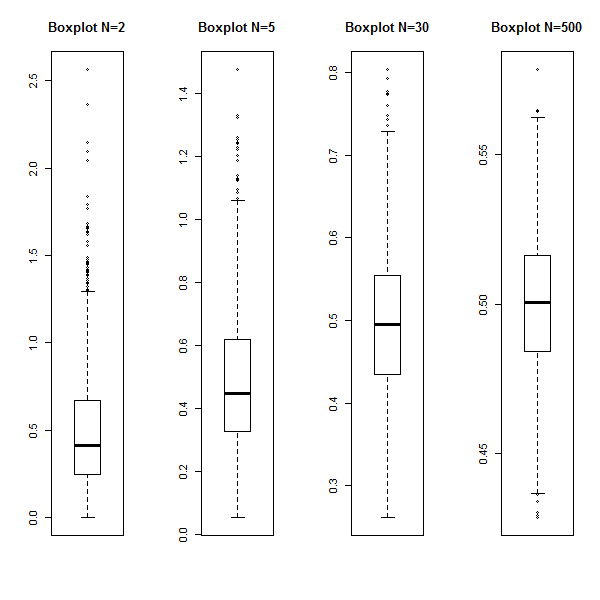
\includegraphics[scale = 1]{grafico15}}
	\end{figure}
	
	Luego de ver estos datos podemos inferir lo siguiente, a medida que aumentamos la cantidad de observaciones en cada muestra, estas muestras se acercan cada vez m\'as a la esperanza de la variable, podemos decir entonces que si tomaramos una infinita cantidad de observaciones entonces las muestras deber\'ian converger a la esperanza. De esto mismo habla la Ley de los Grandes N\'umeros, que dice que la media de las observaciones de n variables aleatorias i.i.d. con igual esperanza $\mu$ finita se aproxima en probabilidad a $\mu$.
	
	Adem\'as, medida que aumentamos las observaciones de las muestras, pudemos ver que los gr\'aficos la distribuci\'on de las medias se iba acercando al gr\'afico que le corresponde a una variable aleatoria normal (de par\'ametros desconocidos), entonces si tom\'aramos una infinita cantidad de observaciones podr\'iamos decir que la distribuci\'on de las medias es aproximadamente la de una normal (de par\'ametros desconocidos).
	
	\newpage
	
	\section{Tercer Ejercicio}
	
	Tomando $X_1,...,X_n$ variables aleatorias i.i.d. con distribuci\'on exponencial de par\'ametro $\lambda = 2$, vamos a comprobar que la distribuci\'on de la variable aleatoria $\frac{\bar{X_n} - E(X_1)}{\sqrt{\frac{Var(X_1)}{n}}}$ estandarizada se aproxima a la de una normal estandarizada cuando $n$ es grande.
	Primero veamos $E(X_1)$ y $Var(X_1)$, como sabemos que $\lambda = 2$ entonces $E(X_1) = \frac{1}{\lambda} = \frac{1}{2}$ y $Var(X_1) = \frac{1}{\lambda^2} = \frac{1}{4}$.
	\smallskip
	
	Ahora si estandarizamos los conjuntos de variables aleatorias del ejercicio anterior, obtenemos como resultando los siguientes gr\'aficos:
	
	\begin{figure}[H]
		\centering
		\subfloat{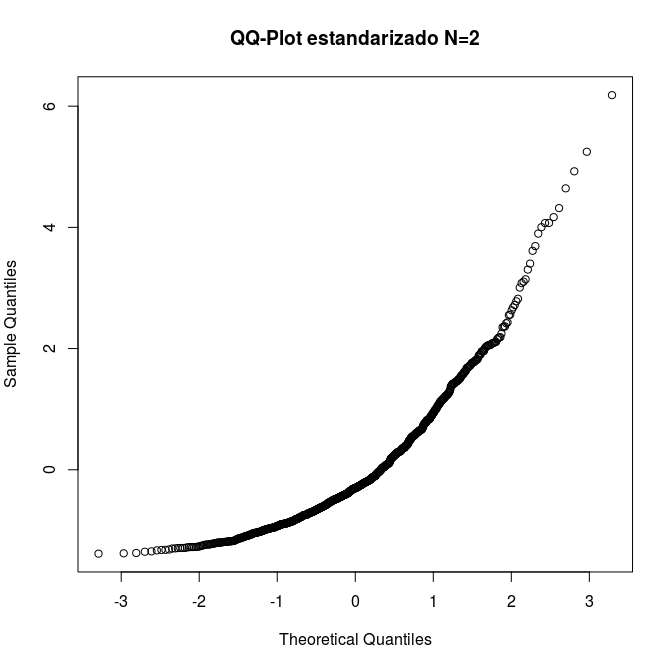
\includegraphics[scale = 0.3]{grafico16}}
		\hfill
		\subfloat{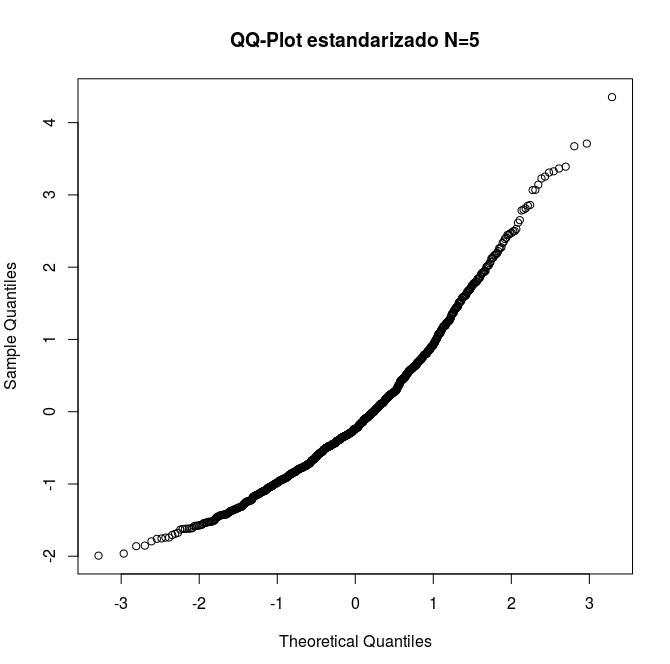
\includegraphics[scale = 0.3]{grafico17}}
	\end{figure}
	
	\begin{figure}[H]
		\centering
		\subfloat{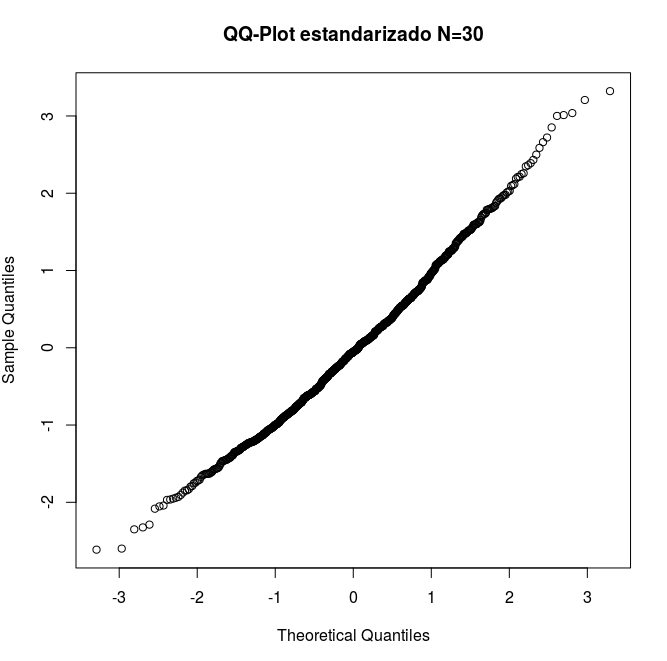
\includegraphics[scale = 0.3]{grafico18}}
		\hfill
		\subfloat{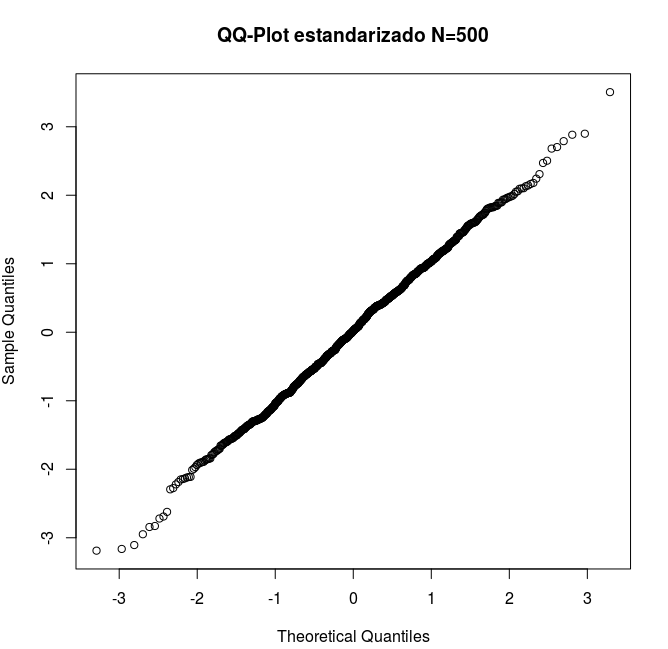
\includegraphics[scale = 0.3]{grafico19}}
	\end{figure}
	
	En estos QQ-plots se puede ver que a medida que $n$ se hace m\'as grande, la distribuci\'on de la variable estandarizada se parece m\'as a la de una normal est\'andar de par\'ametros $\mu = 0$ y $\sigma^2 = 1$.
	Observando los siguientes boxplots tambi\'en podemos ver que la distribuci\'on se vuelve m\'as sim\'etrica a medida que aumenta $n$:
	
	\begin{figure}[H]
		\centering
		\subfloat{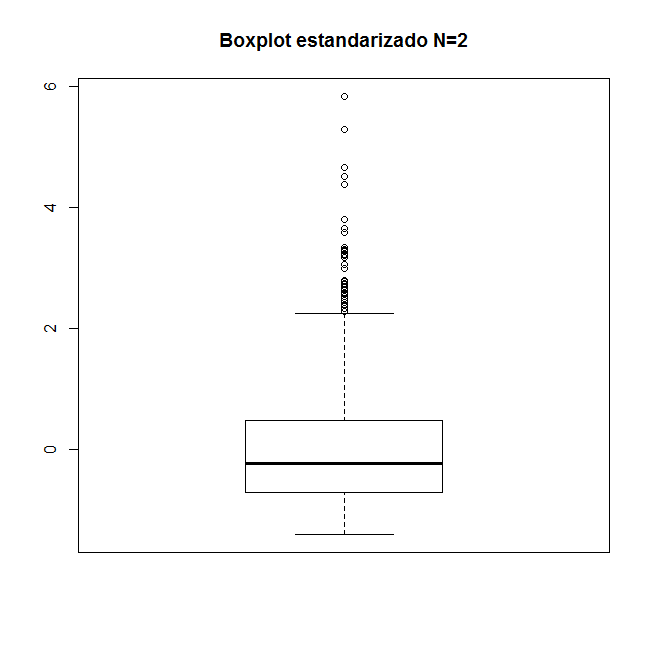
\includegraphics[scale = 0.45]{grafico20}}
		\hfill
		\subfloat{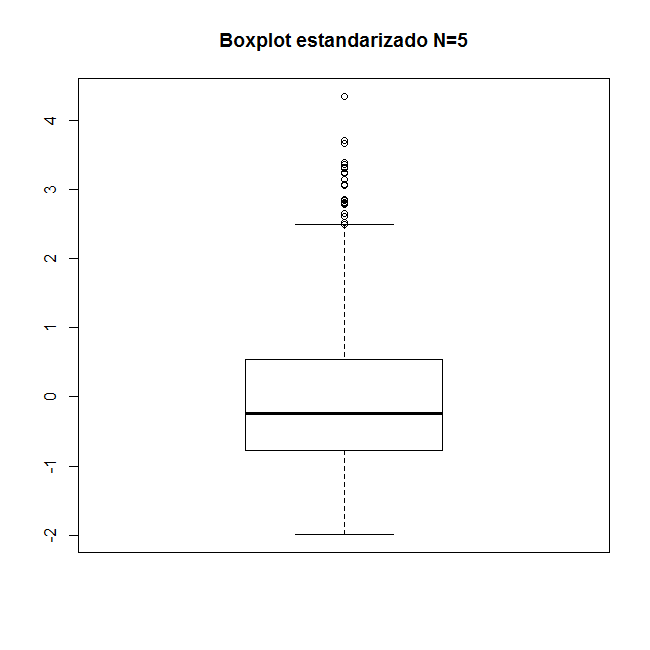
\includegraphics[scale = 0.45]{grafico21}}
	\end{figure}
	
	\begin{figure}[H]
		\centering
		\subfloat{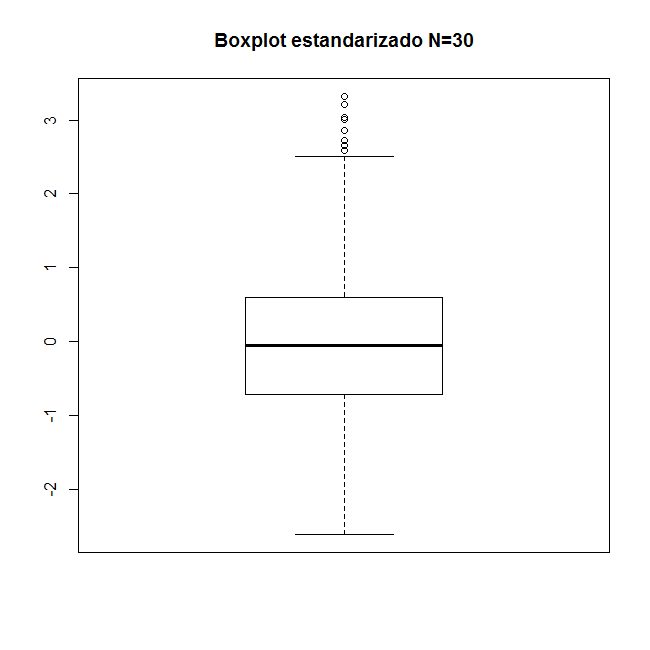
\includegraphics[scale = 0.45]{grafico22}}
		\hfill
		\subfloat{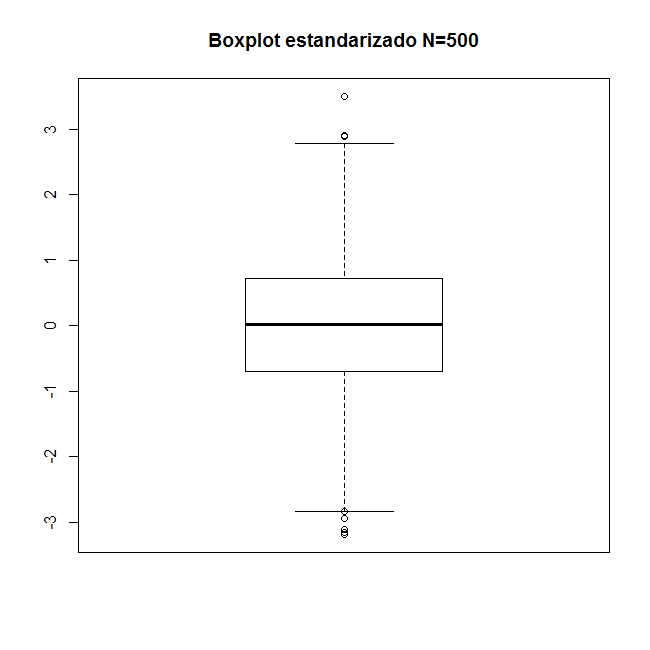
\includegraphics[scale = 0.45]{grafico23}}
	\end{figure}
	
	Finalmente si vemos los histogramas con una funci\'on normal est\'andar superpuesta encima, se puede apreciar como el gr\'afico se asemeja cada vez m\'as a medida que crece la $n$:
	
	\begin{figure}[H]
		\centering
		\subfloat{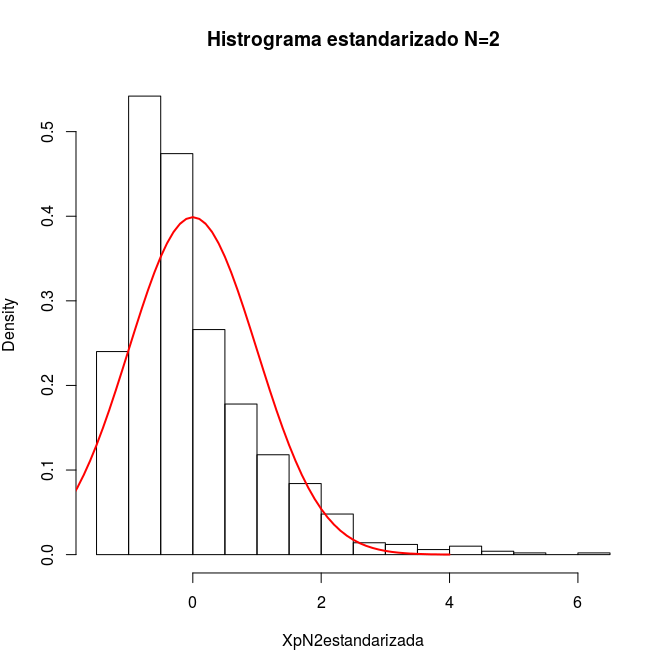
\includegraphics[scale = 0.26]{grafico24}}
		\hfill
		\subfloat{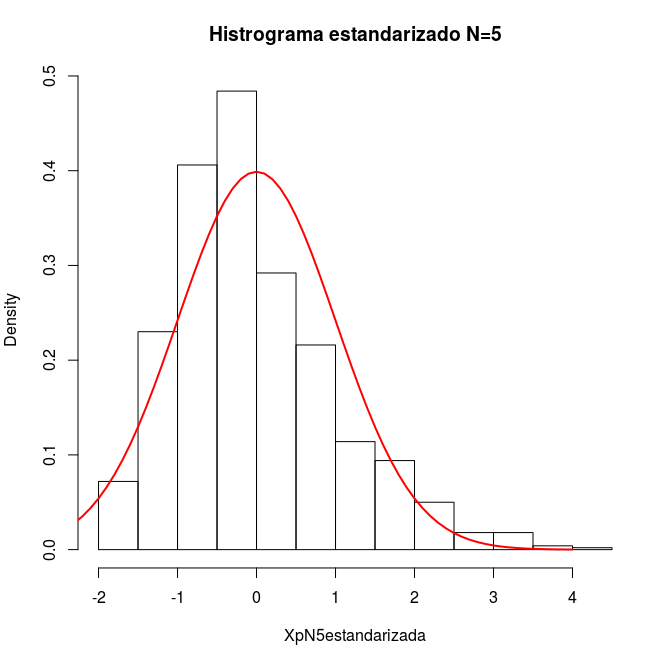
\includegraphics[scale = 0.26]{grafico25}}
	\end{figure}
	
	\begin{figure}[H]
		\centering
		\subfloat{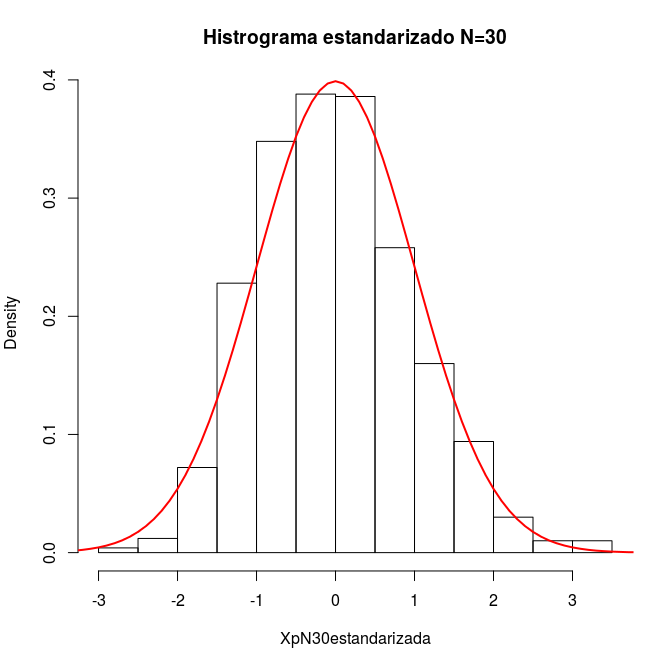
\includegraphics[scale = 0.3]{grafico26}}
		\hfill
		\subfloat{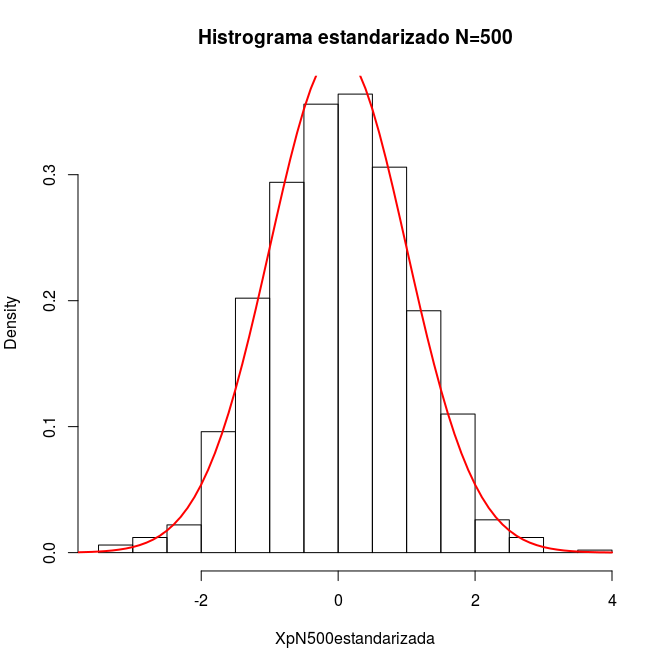
\includegraphics[scale = 0.3]{grafico27}}
	\end{figure}
	
	\newpage
	
	\section{Cuarto Ejercicio}
	
	Para mostrar que la Ley de los Grandes N\'umeros y el Teorema Central del L\'imite no necesariamente son \'unicos de las variables continuas, vamos a realizar los ejercicios anteriores cambiando la distribuci\'on de las variables aleatorias usadas con una diferente y veremos que los resultados son similares.
	La nueva distribuci\'on de las variables aleatorias va a ser una binomial de par\'ametros $n = 6$ y $p = \frac{1}{9}$.
	
	\subsection{Primer Ejercicio Modificado}
	
	Realizando el mismo experimento que el primer ejercicio terminamos con los siguientes gr\'aficos:
	
	\begin{figure}[H]
		\centering
		\subfloat{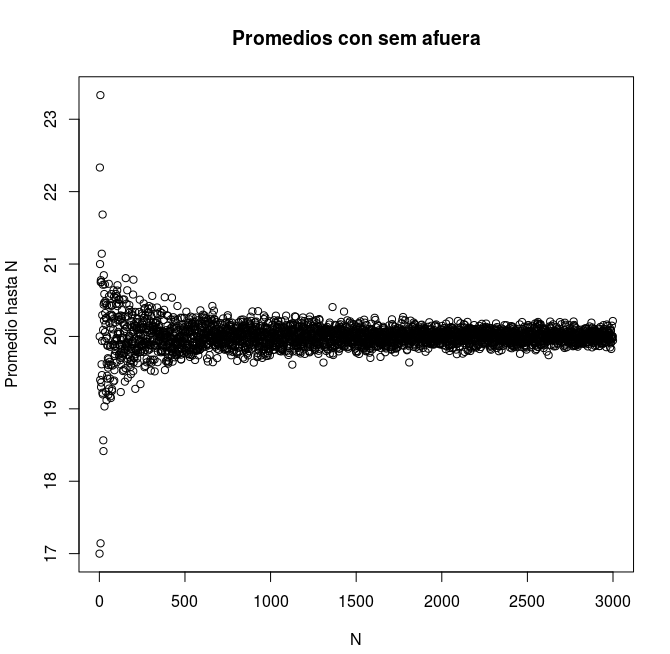
\includegraphics[scale = 0.3]{grafico28}}
		\hfill
		\subfloat{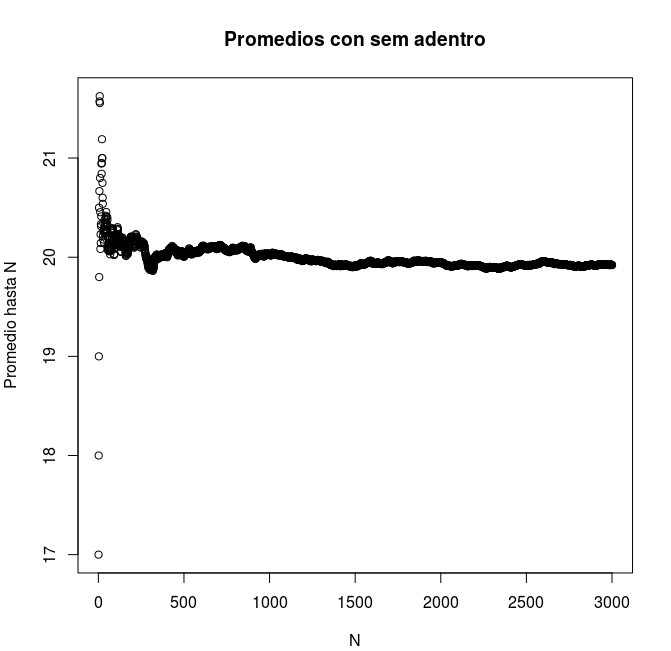
\includegraphics[scale = 0.3]{grafico29}}
	\end{figure}
	
	Podemos ver que pese a que cambiamos la distribuci\'on dela variable aleatoria utilizada por una discreta, terminamos con gr\'aficos que tienen caracter\'isticas similares a las del primer ejercicio original. El gr\'afico que tiene la semilla afuera converge a la esperanza de una variable aleatoria binomial de par\'ametros $n = 6$ y $p = \frac{1}{9}$ y el gr\'afico con la semilla afuera funciona de forma id\'entica al del ejercicio original.
	
	\subsection{Segundo Ejercicio Modificado}
	
	Cambiando la distribuci\'on de la variable en este experimento, algunos gr\'aficos son un poco distintos pero a\'un asi se comportan de forma similar. Veamos los QQ-plot primero:
	
	\begin{figure}[H]
		\centering
		\subfloat{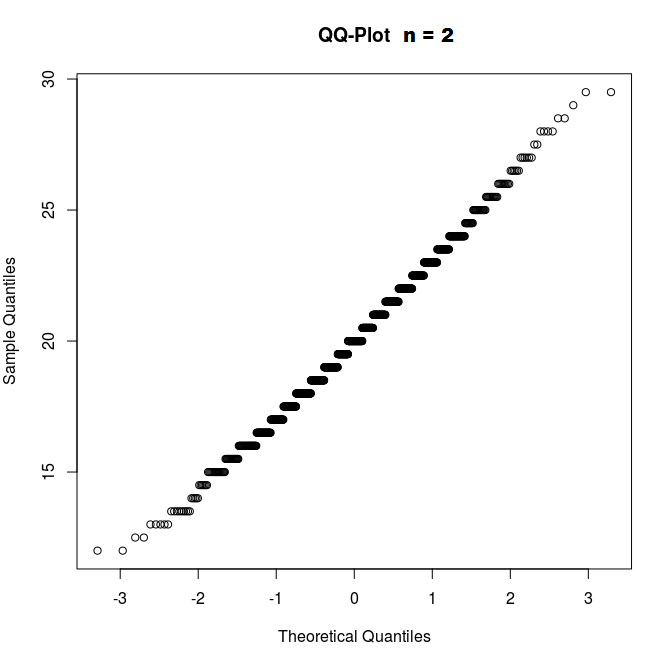
\includegraphics[scale = 0.4]{grafico30}}
		\hfill
		\subfloat{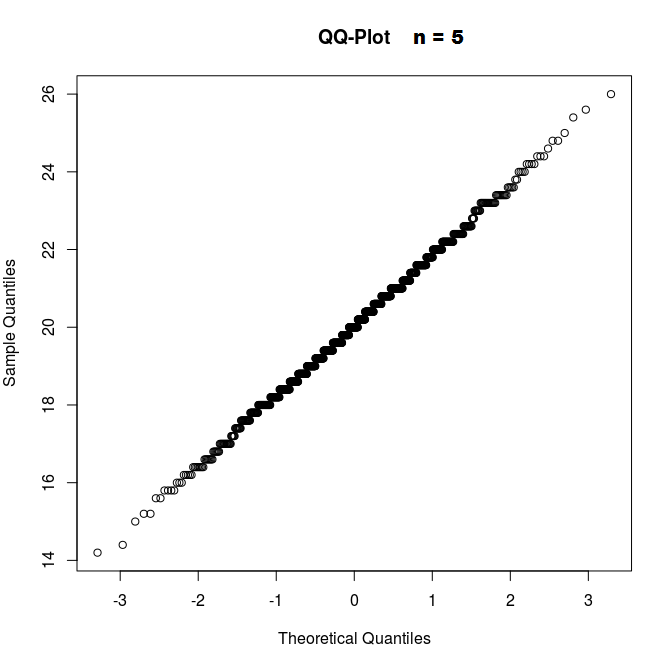
\includegraphics[scale = 0.4]{grafico31}}
	\end{figure}
	
	\begin{figure}[H]
		\centering
		\subfloat{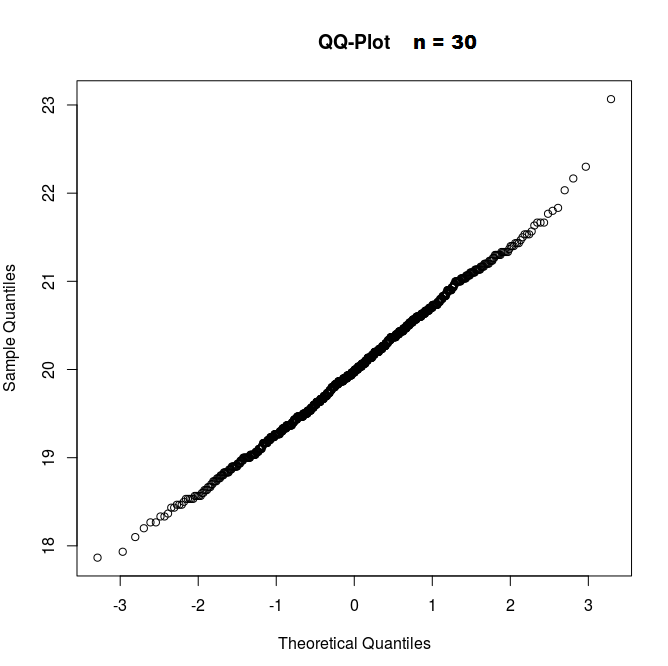
\includegraphics[scale = 0.4]{grafico32}}
		\hfill
		\subfloat{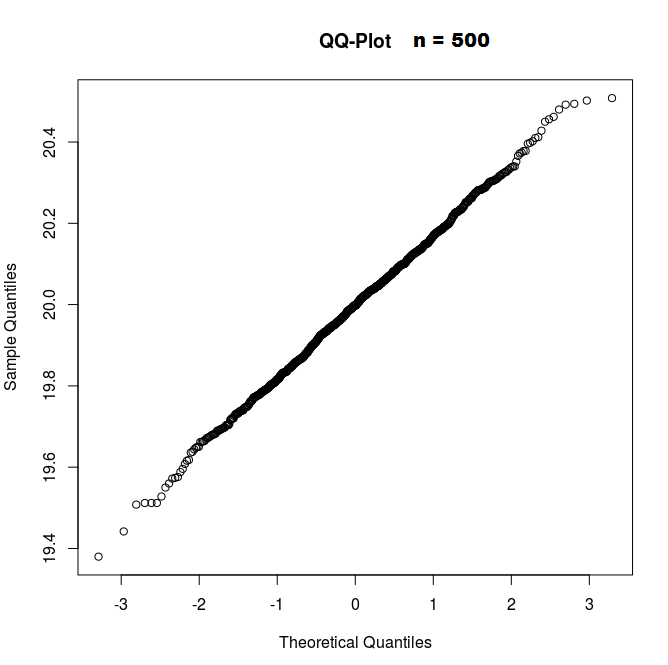
\includegraphics[scale = 0.4]{grafico33}}
	\end{figure}
	
	Podemos ver que al aumentar el $n$, la distribuci\'on se va pareciendo m\'as a una normal como sucedi\'o el segundo ejercicio.
	
	Si vemos los histogramas tambi\'en se nota un comportamiento similar al del segundo ejercicio:
	
	\begin{figure}[H]
		\centering
		\subfloat{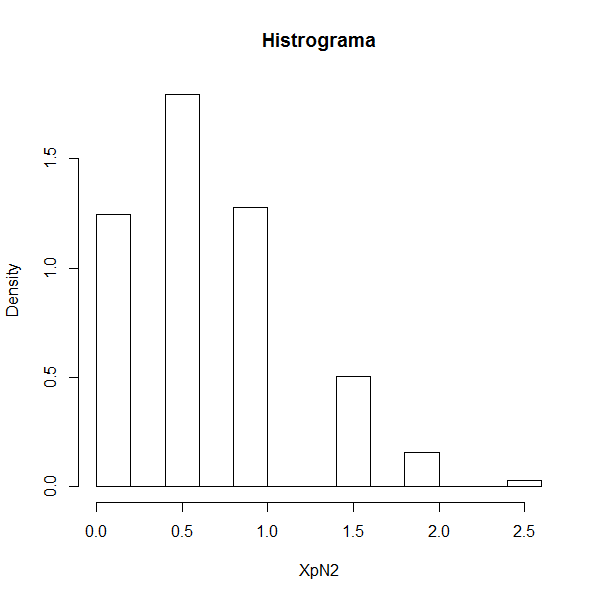
\includegraphics[scale = 0.4]{grafico34}}
		\hfill
		\subfloat{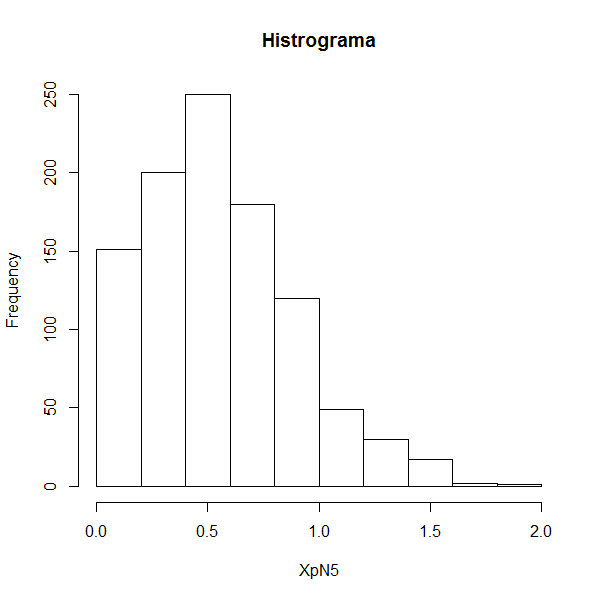
\includegraphics[scale = 0.4]{grafico35}}
	\end{figure}
	
	\begin{figure}[H]
		\centering
		\subfloat{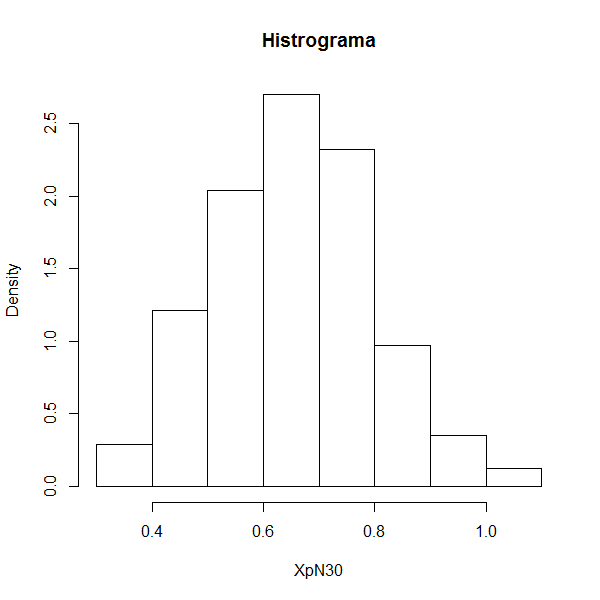
\includegraphics[scale = 0.4]{grafico36}}
		\hfill
		\subfloat{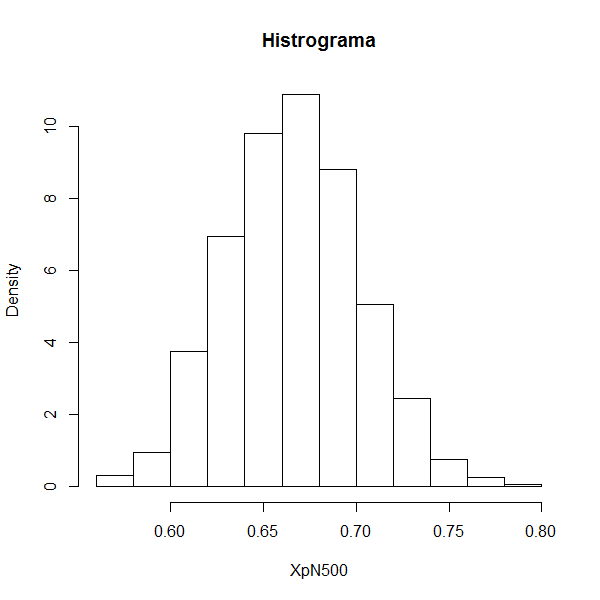
\includegraphics[scale = 0.4]{grafico37}}
	\end{figure}
	
	Vemos que los gr\'aficos se parecen a los de una normal a medida que aumentamos la $n$, tambi\'en vemos que cada ves que aumenta $n$, las muestras se acercan al valor de la esperanza.
	
	Finalmente viendo los boxplots, vemos que tambi\'en se centran a medida que el $n$ se vuelve m\'as grande, pareci\'endose al boxplot de una normal.
	
	\begin{figure}[H]
		\centering
		\subfloat{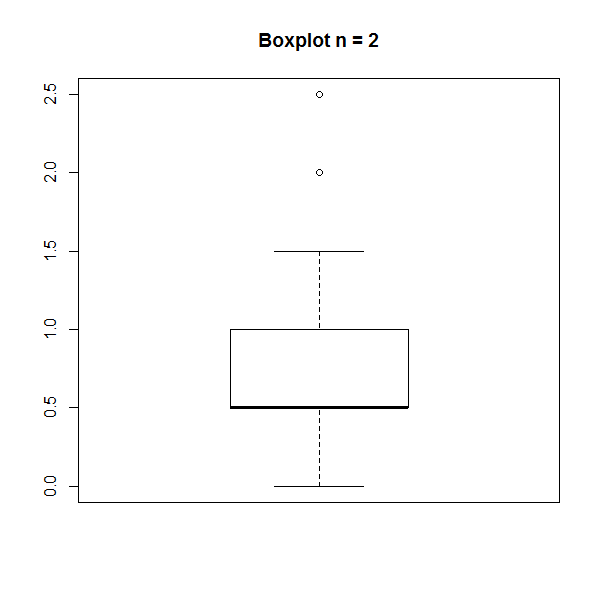
\includegraphics[scale = 0.45]{grafico38}}
		\hfill
		\subfloat{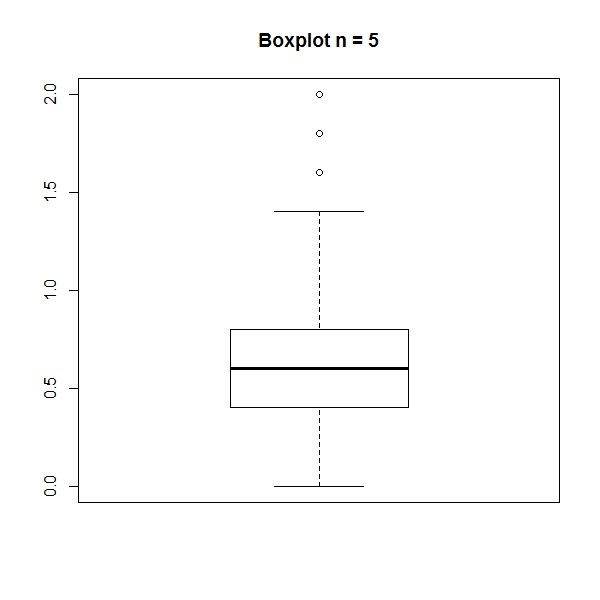
\includegraphics[scale = 0.45]{grafico39}}
	\end{figure}
	
	\begin{figure}[H]
		\centering
		\subfloat{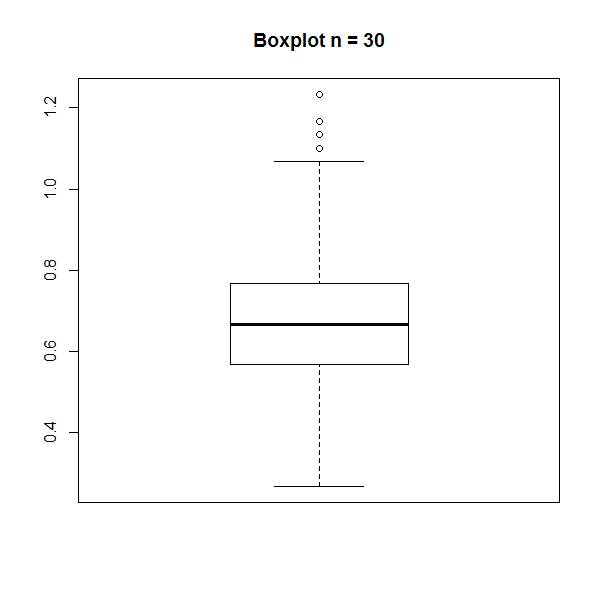
\includegraphics[scale = 0.45]{grafico40}}
		\hfill
		\subfloat{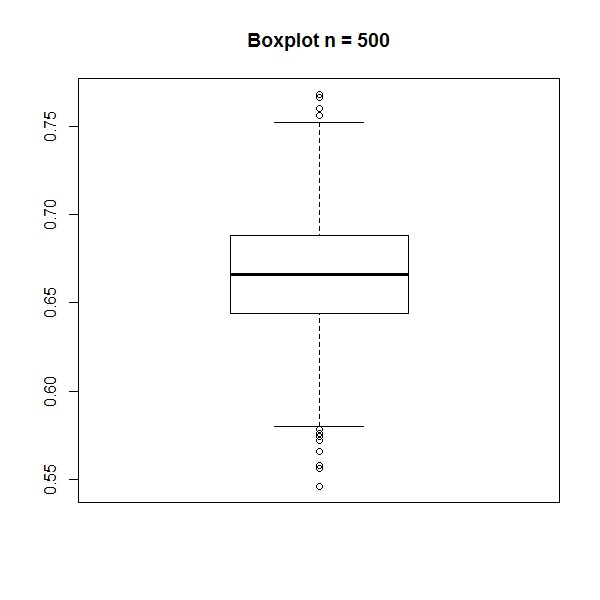
\includegraphics[scale = 0.45]{grafico41}}
	\end{figure}
	
	\subsection{Tercer Ejercicio Modificado}
	
	Si estandarizamos las variables con distribuci\'on binomial de la misma forma que hicimos en el tercer ejercico original obtenemos los siguientes gr\'aficos:
	
	\begin{figure}[H]
		\centering
		\subfloat{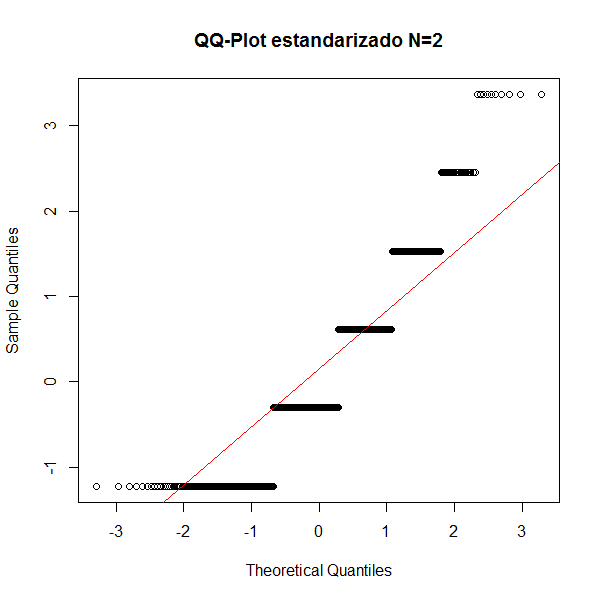
\includegraphics[scale = 0.4]{grafico42}}
		\hfill
		\subfloat{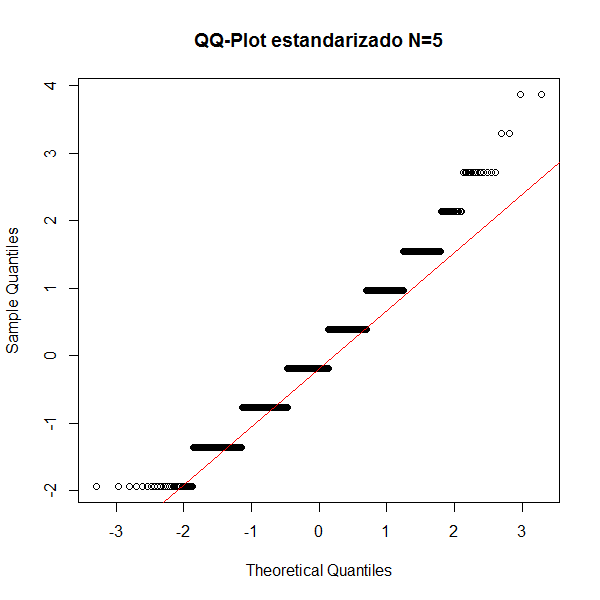
\includegraphics[scale = 0.4]{grafico43}}
	\end{figure}
	
	\begin{figure}[H]
		\centering
		\subfloat{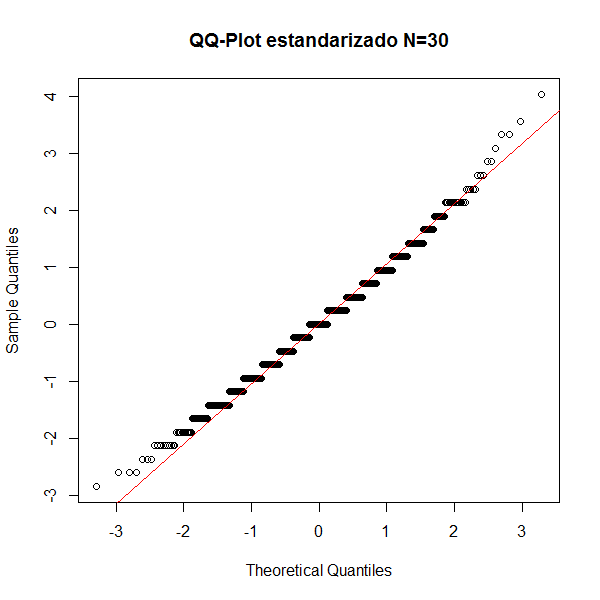
\includegraphics[scale = 0.45]{grafico44}}
		\hfill
		\subfloat{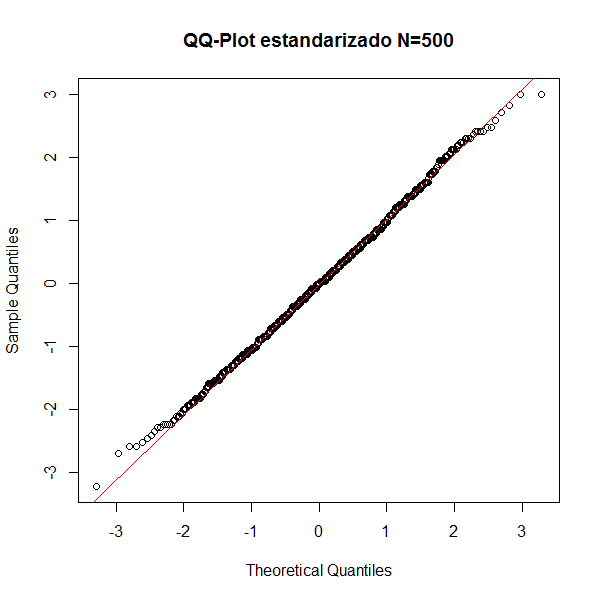
\includegraphics[scale = 0.45]{grafico45}}
	\end{figure}
	
	Se puede ver que mientras más aumenta la $n$, el gr\'afico se parece cada ves m\'as a la recta que seguir\'ia una normal de par\'ametros $\mu = 0$ y $\sigma^2 = 1$.
	
	Los boxplots de los experimentos se ven de la siguiente forma:
	
	\begin{figure}[H]
		\centering
		\subfloat{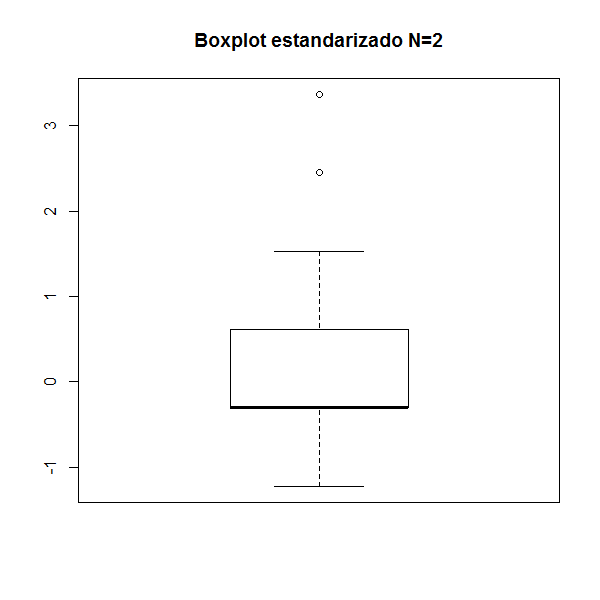
\includegraphics[scale = 0.4]{grafico46}}
		\hfill
		\subfloat{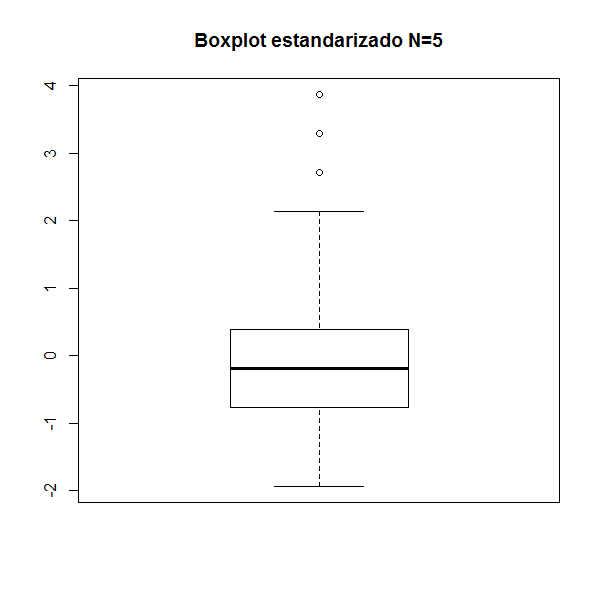
\includegraphics[scale = 0.4]{grafico47}}
	\end{figure}
	
	\begin{figure}[H]
		\centering
		\subfloat{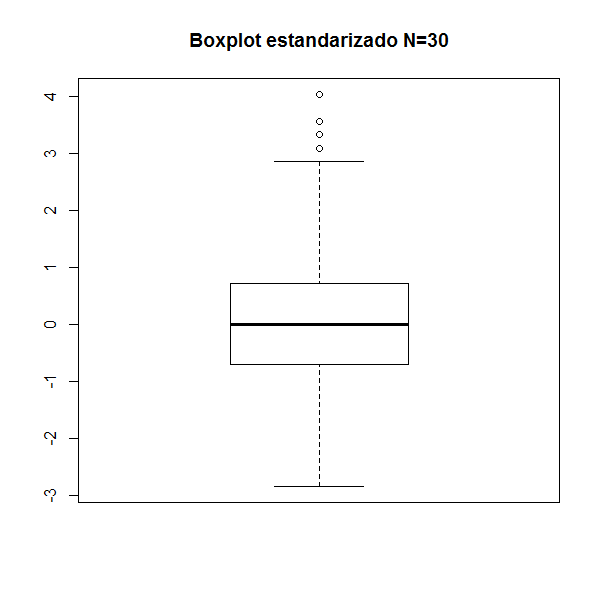
\includegraphics[scale = 0.45]{grafico48}}
		\hfill
		\subfloat{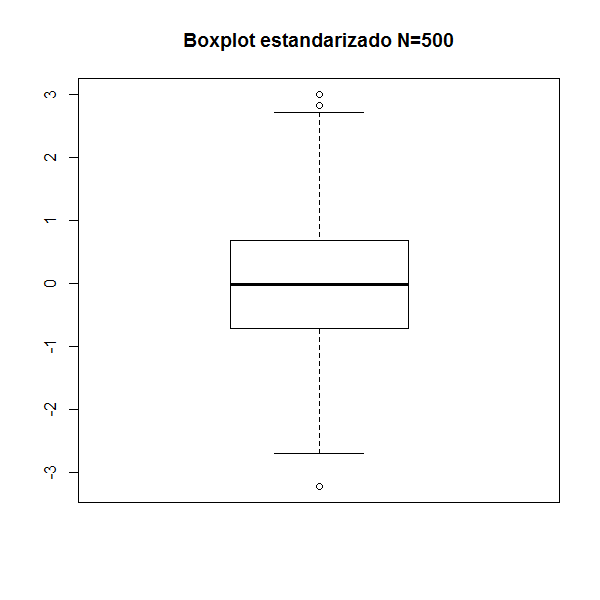
\includegraphics[scale = 0.45]{grafico49}}
	\end{figure}
	
	Podemos ver que los boxplots tambi\'en se parecen a los de una normal de par\'ametros $\mu = 0$ y $\sigma^2 = 1$ a medida que $n$ aumenta.
	
	Finalmente viendo los histogramas:
	
	\begin{figure}[H]
		\centering
		\subfloat{\includegraphics[scale = 0.3]{grafico50}}
		\hfill
		\subfloat{\includegraphics[scale = 0.3]{grafico51}}
	\end{figure}
	
	\begin{figure}[H]
		\centering
		\subfloat{\includegraphics[scale = 0.3]{grafico52}}
		\hfill
		\subfloat{\includegraphics[scale = 0.3]{grafico53}}
	\end{figure}
	
	Podemos ver que a medida que aumenta $n$, el gr\'afico se parece cada vez m\'as el de una normal de par\'ametros $\mu = 0$ y $\sigma^2 = 1$. 

%	\newpage
	
%	\section{Conclusiones}
%	
%	\newpage

\end{document}
